\chapter{Entwurfsmuster}
\label{entwurfsmuster}
Innerhalb dieses Kapitels werden die Umsetzung von \textit{Entwurfsmustern} innerhalb des Softwareentwurfs analysiert und deren Verwendung begründet.

%\section{Betrachtete Entwurfsmuster}
%\todo[]{Bridge}
%\todo[]{Builder}
%\todo[]{Singleton / IOC}
%\todo[]{Observer - es muss kein neuer Observer programmiert werden, es reicht aus, wenn er verwendet wird und das entsprechend durch UML-Diagramm gezeigt wird}

\section{Angewandte Entwurfsmuster}
Bei Betrachtung der Ausschnitte aus dem \href{https://github.com/lucasmerkel/dhbw-advancedswe-programmentwurf/blob/d5c89113d12c3b877ddc4d6a99225b277ddd468f/Documentation/Bilder/uml-diagramme/klassendiagramm.svg}{\code{UML-Diagramm}} ist der \href{https://github.com/lucasmerkel/dhbw-advancedswe-programmentwurf/blob/2bab7b1c200507e4550ce7025485261d0e95ce07/Documentation/Bilder/uml-diagramme/uml-entwurfsmuster-builder.svg}{\textit{Builder}} in Abbildung \ref{fig:uml-builder-pattern} sowie die \href{https://github.com/lucasmerkel/dhbw-advancedswe-programmentwurf/blob/d5c89113d12c3b877ddc4d6a99225b277ddd468f/Documentation/Bilder/uml-diagramme/uml-entwurfsmuster-bridge.svg}{\textit{Bridge}} in Abbildung \ref{fig:uml-bridge-pattern} als Entwurfsmuster zu erkennen, die in diesem Softwareentwurf angewandt wurden.

\begin{figure}[H]
 	\centering
 	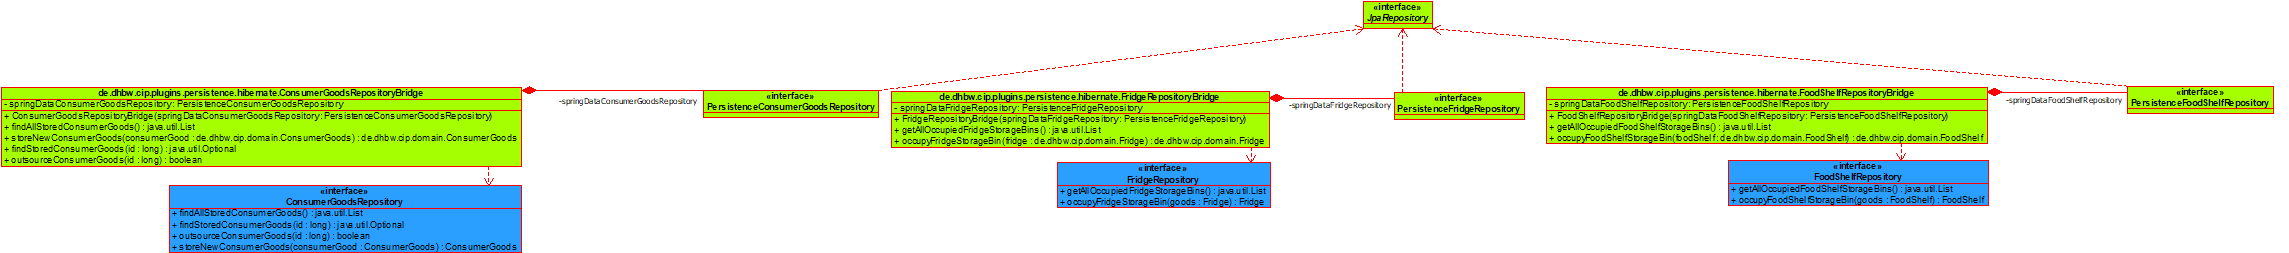
\includegraphics[width=1.0\textwidth]{Bilder/uml-diagramme/entwurfsmuster-bridge.png}
 	\caption[Ausschnitt des UML-Diagramms zur Darstellung des \textit{Bridge}-Entwurfmusters.]{Der Ausschnitt des UML-Diagramms verdeutlicht die Verwendung des \textit{Bridge}-Entwurfmusters.}
 	\label{fig:uml-bridge-pattern}
 \end{figure}

 \begin{figure}[H]
 	\centering
 	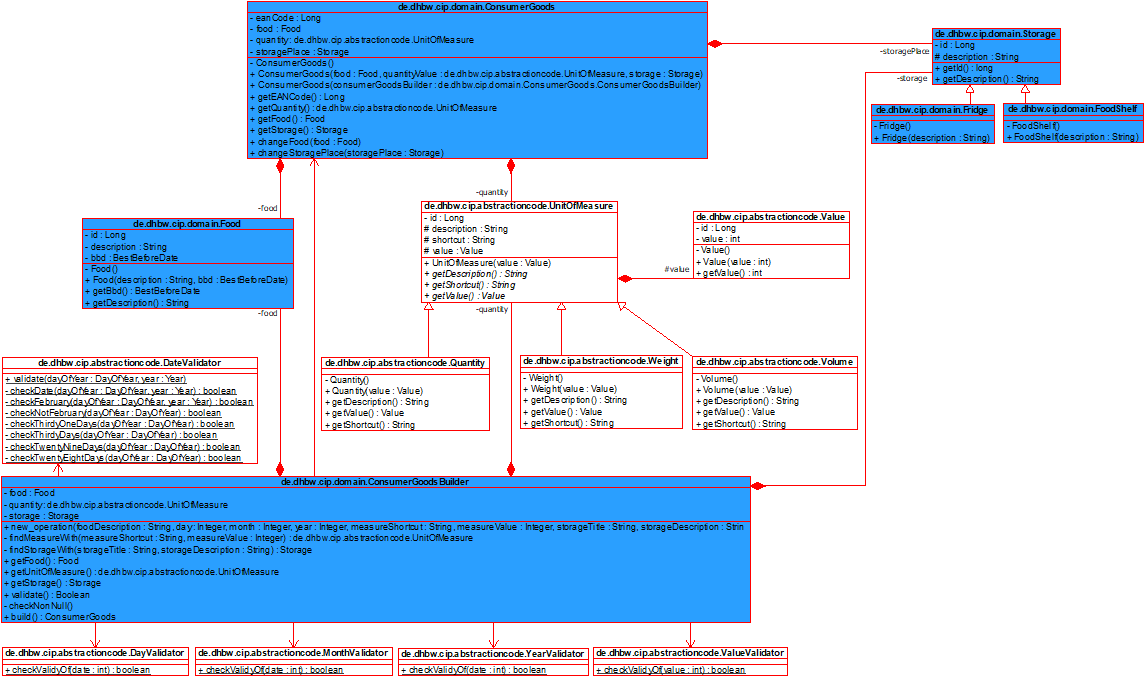
\includegraphics[width=1.0\textwidth]{Bilder/uml-diagramme/entwurfsmuster-builder.png}
 	\caption[Ausschnitt des UML-Diagramms zur Darstellung des \textit{Builder}-Entwurfmusters.]{Der Ausschnitt des UML-Diagramms verdeutlicht die Verwendung des \textit{Builder}-Entwurfmusters.}
 	\label{fig:uml-builder-pattern}
 \end{figure}

\subsection*{\textit{Builder}-Entwurfsmuster}
Das \textit{Builder}-Entwurfsmuster zählt zu den \textit{Erzeugungsmustern} und ist in der Klasse \href{https://github.com/lucasmerkel/dhbw-advancedswe-programmentwurf/blob/d5c89113d12c3b877ddc4d6a99225b277ddd468f/swe_programmentwurf/consumergoods-inventory-planner/3-cip-domain/src/main/java/de/dhbw/cip/domain/ConsumerGoods.java#L72}{\code{ConsumerGoodsBuilder}} umgesetzt.
An dieser Stelle wurde ein \textit{Builder}-Entwurfsmuster eingesetzt, da es die Möglichkeit gibt, nötige Attribute zu sammeln und, im Gegensatz zum direkten Erzeugen eines Objekts, die Möglichkeit der Überprüfung auf Gültigkeit der Attribute vor dem Erzeugen des Objekts ermöglicht.
Der Einsatz ist in diesem Fall sinnvoll, da neben dem Abfangen von Fehlern bei der fehlenden Übertragung von Attributen, Datumseingaben oder Werteeingaben diese auf Gültigkeit zu überprüfen sind.

Das \textit{Bridge}-Entwurfsmuster zählt zu den \textit{Strukturmustern} und ist in den Klassen \href{https://github.com/lucasmerkel/dhbw-advancedswe-programmentwurf/blob/d5c89113d12c3b877ddc4d6a99225b277ddd468f/swe_programmentwurf/consumergoods-inventory-planner/0-cip-plugins/src/main/java/de/dhbw/cip/plugins/persistence/hibernate/ConsumerGoodsRepositoryBridge.java}{\code{ConsumerGoodRepositoryBridge}}, \href{https://github.com/lucasmerkel/dhbw-advancedswe-programmentwurf/blob/d5c89113d12c3b877ddc4d6a99225b277ddd468f/swe_programmentwurf/consumergoods-inventory-planner/0-cip-plugins/src/main/java/de/dhbw/cip/plugins/persistence/hibernate/FridgeRepositoryBridge.java}{\code{FridgeRepositoryBridge}} sowie \\\href{https://github.com/lucasmerkel/dhbw-advancedswe-programmentwurf/blob/d5c89113d12c3b877ddc4d6a99225b277ddd468f/swe_programmentwurf/consumergoods-inventory-planner/0-cip-plugins/src/main/java/de/dhbw/cip/plugins/persistence/hibernate/FoodShelfRepositoryBridge.java}{\code{FoodShelfRepositoryBridge}} umgesetzt.
Das \textit{Bridge}-Entwurfsmuster wurde eingesetzt, da es die Trennung der Domänenlogik von der Pluginlogik ermöglicht.
Während die Repository-Interfaces \\\href{https://github.com/lucasmerkel/dhbw-advancedswe-programmentwurf/blob/619ca36fff0fa0b6633ecae25c098e1252993086/swe_programmentwurf/consumergoods-inventory-planner/3-cip-domain/src/main/java/de/dhbw/cip/domain/ConsumerGoodsRepository.java}{\code{ConsumerGoodRepository}}, \href{https://github.com/lucasmerkel/dhbw-advancedswe-programmentwurf/blob/619ca36fff0fa0b6633ecae25c098e1252993086/swe_programmentwurf/consumergoods-inventory-planner/3-cip-domain/src/main/java/de/dhbw/cip/domain/FridgeRepository.java}{\code{FridgeRepository}} und \href{https://github.com/lucasmerkel/dhbw-advancedswe-programmentwurf/blob/619ca36fff0fa0b6633ecae25c098e1252993086/swe_programmentwurf/consumergoods-inventory-planner/3-cip-domain/src/main/java/de/dhbw/cip/domain/FoodShelfRepository.java}{\code{FoodShelfRepository}} zur Domäne zählen, findet die Persistierung der Objekte über ein Plugin mit der Implementierung der Interfaces \href{https://github.com/lucasmerkel/dhbw-advancedswe-programmentwurf/blob/d5c89113d12c3b877ddc4d6a99225b277ddd468f/swe_programmentwurf/consumergoods-inventory-planner/0-cip-plugins/src/main/java/de/dhbw/cip/plugins/persistence/hibernate/PersistenceConsumerGoodsRepository.java}{\code{PersistenceConsumerGoodRepository}}, \\\href{https://github.com/lucasmerkel/dhbw-advancedswe-programmentwurf/blob/d5c89113d12c3b877ddc4d6a99225b277ddd468f/swe_programmentwurf/consumergoods-inventory-planner/0-cip-plugins/src/main/java/de/dhbw/cip/plugins/persistence/hibernate/PersistenceFridgeRepository.java}{\code{PersistenceFridgeRepository}} sowie \href{https://github.com/lucasmerkel/dhbw-advancedswe-programmentwurf/blob/d5c89113d12c3b877ddc4d6a99225b277ddd468f/swe_programmentwurf/consumergoods-inventory-planner/0-cip-plugins/src/main/java/de/dhbw/cip/plugins/persistence/hibernate/PersistenceFoodShelfRepository.java}{\code{PersistenceFoodShelfRepository}} statt.
Durch Anwenden des \textit{Bridge}-Entwurfsmuster ist es nun möglich, auf einen implementierten Typ des entsprechenden Repository-Interfaces für die Interaktion mit der Entitätsverwaltung zuzugreifen.
Das \textit{Bridge}-Entwurfsmuster hat das entsprechende Repository-Interface implementiert und übernimmt die Kommunikation mit dem Persistierungs-Plugin.
Somit ist die Aufteilung entsprechend der \textit{Clean Architecture} gewährleistet und bei einem Austausch des Persistierungs-Plugins bedarf es nur Änderungen in der \textit{Plugin}-Schicht, während das Repository-Interface in der \textit{Domänen}-Schicht sowie alle darauf zugreifenden Instanzen davon unberührt sind.
